\documentclass[compress]{beamer}
\usetheme{Warsaw}
\usecolortheme{seagull}
\setbeamertemplate{headline}{}
\beamertemplatenavigationsymbolsempty

\usepackage{lipsum}
\setbeamersize{text margin left=10pt,text margin right=10pt}

\addtobeamertemplate{navigation symbols}{}{%
    \usebeamerfont{footline}%
    \usebeamercolor[fg]{footline}%
    \hspace{1em}%
    \insertframenumber/\inserttotalframenumber
}

\usepackage{graphicx}
\graphicspath{{/Users/jlochman/Desktop/Diploma-thesis/Chapter3/}}
\usepackage{epstopdf}
\usepackage{booktabs} 
\usepackage{courier}

\PassOptionsToPackage{demo}{graphicx}
\def\Put(#1,#2)#3{\leavevmode\makebox(0,0){\put(#1,#2){#3}}}


\title[Unfolding Approaches]{Comparison of Two Unfolding Approaches} 
\author{Jan Lochman}
\institute[FNSPE CTU] 
{
Czech Technical University \\ 
\medskip
\textit{jan.lochman@cern.ch} \\
\medskip
\medskip
Inclusive Jet Meeting \\ 
\medskip
}
\date{\today}

\begin{document}

%------------------------------------------------

\begin{frame}
\titlepage 
\end{frame}

%------------------------------------------------

%\begin{frame}
%\frametitle{Overview} 
%\tableofcontents 
%\end{frame}

\begin{frame}
\frametitle{Introduction}
\begin{itemize}
  \item Double differential inclusive jet cross section in $p_T$ and $|y|$
  \item \textbf{Data} 
    \begin{itemize}
      \item \texttt{mc14\_13TeV, AntiKt4LCTopoJets}
    \end{itemize}
  \item \textbf{Event Selection}
    \begin{itemize}
      \item $p_T>15\,\text{GeV}$, $|y|<4$ 
      \item \# reco jets $\geq 1$ \& \# truth jets $\geq 1$ 
      \item $0.6 < p_{T,leading}^{reco} / p_{T,leading}^{truth} < 1.4$.
    \end{itemize}
  \item \textbf{Jet matching}
    \begin{itemize}
      \item Angular matching starting from lowest $dR_{ij}$
      \item $dR_{ij} = \sqrt{d\phi_{ij}^2 + dy_{ij}^2} < 0.2$
    \end{itemize}
\end{itemize}
\end{frame}

\begin{frame}
\frametitle{Introduction to Unfolding}
\begin{itemize}
  \item Used two approaches to unfolding
  \item \textbf{Simple Unfolding}
    \begin{itemize}
      \item Matching only within the same rapidity bins.
      \item 8 transfer matrices 46x46 (8 = \# $y$-Bins, 46 = \# $p_{T}$-Bins).
      \item Unfolding done for each transfer matrix separately.
    \end{itemize}
  \item \textbf{2D Unfolding}
    \begin{itemize}
      \item Matching between different rapidity bins allowed.
      \item 1 transfer matrix 368x368 (368 = 8x46).
    \end{itemize}
  \item \textbf{Differences:}
    \begin{itemize}
      \item Different transfer matrices.
      \item Different matching efficiencies.
    \end{itemize}
\end{itemize}
\end{frame}

%------------------------------------------------

\begin{frame}
\frametitle{Transfer Matrices}
\begin{columns}[onlytextwidth]
  \begin{column}{0.5\textwidth}
    2D unfolding
    \begin{figure}[H]
      \centering
      \includegraphics[width=\textwidth]{{unfold_matrix_all}.eps}
    \end{figure}
  \end{column}
  \begin{column}{0.5\textwidth}
    Simple unfolding
    \begin{figure}[H]
      \centering
      \includegraphics[width=\textwidth]{{unfold_matrix_firstBin}.eps}
    \end{figure}
  \end{column}
\end{columns}
\end{frame}

%------------------------------------------------

\begin{frame}
\frametitle{High $p_T$ Difference in Matched Jets}
\tiny
mc14\_13TeV.147915.Pythia8\_AU2CT10\_jetjet\_JZ5W.merge.AOD.e2743\_s1982\_s2008\_r5787\_r5853/
\quad   AOD.01598029.\_000003.pool.root.1  \quad  event \# 1087   \quad (left)

mc14\_13TeV.147916.Pythia8\_AU2CT10\_jetjet\_JZ6W.merge.AOD.e2743\_s1982\_s2008\_r5787\_r5853/
\quad   AOD.01598030.\_000005.pool.root.2  \quad  event \# 1388   \quad (right)

\begin{columns}[onlytextwidth]
  \begin{column}{0.5\textwidth}
    \begin{table}
      \begin{tabular}{l l l l}
        \toprule
        \textbf{Jet Level} & $\mathbf{p_T}$ & $\mathbf{y}$ & $\mathbf{\phi}$ \\
        \midrule
        RECO  &  1948.9 &  0.7973 &  -2.996 \\
        TRUTH &  1913.0 &  0.8159 &  -2.996 \\
        \midrule 
        RECO  &  1526.4 &  -0.686 &  0.1032 \\
        TRUTH &  1851.6 &  -0.674 &  0.1646 \\
        \midrule 
        \textcolor{red}{RECO}  &  \textcolor{red}{330.04} &  -0.732 &  0.5231 \\
        \textcolor{red}{TRUTH} &  \textcolor{red}{30.748} &  -0.839 &  0.5972 \\
        \midrule
        RECO  &  101.92 &  -0.271 &  -0.133 \\
        TRUTH &  97.678 &  -0.266 &  -0.116 \\
        \midrule 
        RECO  &  55.632 &  -0.086 &  -2.942 \\
        TRUTH &  52.407 &  -0.014 &  -2.905 \\
        \midrule 
        RECO  &  17.514 &  -2.471 &  -2.271 \\
        TRUTH &  25.189 &  -2.472 &  -2.377 \\
        \midrule
        \midrule
        RECO  &  19.760 &  -1.650 &  2.6354 \\
        RECO  &  19.303 &  -0.242 &  -1.035 \\
        RECO  &  17.814 &  0.4432 &  2.8272 \\
        RECO  &  16.998 &  1.8389 &  0.9921 \\
        RECO  &  15.435 &  -0.692 &  -2.578 \\
        \bottomrule
      \end{tabular}
    \end{table}
  \end{column}
  \begin{column}{0.5\textwidth}
    \begin{table}
      \begin{tabular}{l l l l}
        \toprule
        \textbf{Jet Level} & $\mathbf{p_T}$ & $\mathbf{y}$ & $\mathbf{\phi}$ \\
        \midrule
        RECO  &  1468.5 &  0.1580 &  2.0229 \\
        TRUTH &  1420.1 &  0.1633 &  2.0300 \\
        \midrule
        RECO  &  1267.6 &  0.1966 &  -0.928 \\
        TRUTH &  963.99 &  0.2578 &  -0.857 \\
        \midrule
        RECO  &  177.77 &  2.1969 &  -2.344 \\
        TRUTH &  169.13 &  2.2085 &  -2.349 \\
        \midrule
        RECO  &  112.19 &  2.0599 &  -1.753 \\
        TRUTH &  108.35 &  2.0499 &  -1.759 \\
        \midrule
        RECO  &  56.778 &  1.4397 &  2.0556 \\
        TRUTH &  31.550 &  1.3559 &  2.0508 \\
        \midrule
        \textcolor{red}{RECO}  &  \textcolor{red}{19.091} &  -0.111 &  -1.313 \\
        \textcolor{red}{TRUTH} &  \textcolor{red}{340.94} &  0.0072 &  -1.195 \\
        \midrule
        \midrule
        RECO  &  20.420 &  0.6798 &  -0.871 \\
        RECO  &  19.792 &  0.3520 &  -1.622 \\
        \bottomrule
      \end{tabular}
    \end{table}
  \end{column}
\end{columns}
\normalsize
\end{frame}

%------------------------------------------------

\begin{frame}
\frametitle{Slices in Transfer Matrix}
\vfill
\Put(280,40){\color{blue}\includegraphics[height=2.5cm]{{unfold_matrix_all}.eps}}
\begin{figure}[H]
  \centering
  \includegraphics[width=0.33\textwidth]{{UnfoldMatrixSlices00}.eps}
  \includegraphics[width=0.33\textwidth]{{UnfoldMatrixSlices11}.eps}
  \includegraphics[width=0.33\textwidth]{{UnfoldMatrixSlices22}.eps}

  \includegraphics[width=0.33\textwidth]{{UnfoldMatrixSlices33}.eps}
  \includegraphics[width=0.33\textwidth]{{UnfoldMatrixSlices44}.eps}
  \includegraphics[width=0.33\textwidth]{{UnfoldMatrixSlices55}.eps}
\end{figure}
\end{frame}

%------------------------------------------------

\begin{frame}
\frametitle{Matching Efficiencies}
\framesubtitle{Reco Jets}
\begin{figure}[H]
  \centering
  \includegraphics[width=0.33\textwidth]{{MatchEffSimpe2DSignal0Compare}.eps}
  \includegraphics[width=0.33\textwidth]{{MatchEffSimpe2DSignal1Compare}.eps}
  \includegraphics[width=0.33\textwidth]{{MatchEffSimpe2DSignal2Compare}.eps}

  \includegraphics[width=0.33\textwidth]{{MatchEffSimpe2DSignal3Compare}.eps}
  \includegraphics[width=0.33\textwidth]{{MatchEffSimpe2DSignal4Compare}.eps}
  \includegraphics[width=0.33\textwidth]{{MatchEffSimpe2DSignal5Compare}.eps}
\end{figure}
\end{frame}

%------------------------------------------------

\begin{frame}
\frametitle{Matching Efficiencies}
\framesubtitle{Truth Jets}
\begin{figure}[H]
  \centering
  \includegraphics[width=0.33\textwidth]{{MatchEffSimpe2DTruth0Compare}.eps}
  \includegraphics[width=0.33\textwidth]{{MatchEffSimpe2DTruth1Compare}.eps}
  \includegraphics[width=0.33\textwidth]{{MatchEffSimpe2DTruth2Compare}.eps}

  \includegraphics[width=0.33\textwidth]{{MatchEffSimpe2DTruth3Compare}.eps}
  \includegraphics[width=0.33\textwidth]{{MatchEffSimpe2DTruth4Compare}.eps}
  \includegraphics[width=0.33\textwidth]{{MatchEffSimpe2DTruth5Compare}.eps}
\end{figure}
\end{frame}

%------------------------------------------------

\begin{frame}
\frametitle{Different $y$-bins, $p_T>1000\,\text{GeV}$}
\tiny
mc14\_13TeV.147915.Pythia8\_AU2CT10\_jetjet\_JZ5W.merge.AOD.e2743\_s1982\_s2008\_r5787\_r5853/
\quad   AOD.01598029.\_000003.pool.root.1  
\quad  event \# 959 (left)
\quad  event \# 986 (right)
\begin{columns}[onlytextwidth]
  \begin{column}{0.5\textwidth}
    \begin{table}
      \begin{tabular}{l l l l}
        \toprule
        \textbf{Jet Level} & $\mathbf{p_T}$ & $\mathbf{y}$ & $\mathbf{\phi}$ \\
        \midrule
        \textcolor{red}{RECO}   &  \textcolor{red}{1047.2} & \textcolor{red}{0.50084} &  -0.525  \\
        \textcolor{red}{TRUTH}  &  \textcolor{red}{1043.6} & \textcolor{red}{0.49142} &  -0.515  \\
        \midrule
        RECO   &  919.36 &  -0.8124 &  3.0295  \\
        TRUTH  &  859.44 &  -0.8250 &  3.0283  \\
        \midrule
        RECO   &  202.45 &  0.15152 &  1.5866  \\
        TRUTH  &  209.20 &  0.13535 &  1.5925  \\
        \midrule
        RECO   &  107.19 &  3.20412 &  0.9019  \\
        TRUTH  &  110.20 &  3.20996 &  0.8821  \\
        \midrule
        RECO   &  86.126 &  -1.0504 &  2.4963  \\
        TRUTH  &  94.136 &  -1.0531 &  2.5268  \\
        \midrule
        RECO   &  62.074 &  -1.3096 &  -3.053  \\
        TRUTH  &  52.706 &  -1.2922 &  -3.057  \\
        \midrule
        RECO   &  22.069 &  -0.7635 &  2.0193  \\
        TRUTH  &  31.753 &  -0.8044 &  1.8596  \\
        \midrule
        RECO   &  16.189 &  0.79967 &  2.1690  \\
        TRUTH  &  23.677 &  0.93080 &  2.1237  \\
        \midrule
        \midrule
        TRUTH  &  19.405 &  3.71203 &  1.5590  \\
        \bottomrule
      \end{tabular}
    \end{table}
  \end{column}
  \begin{column}{0.5\textwidth}
    \begin{table}
      \begin{tabular}{l l l l}
        \toprule
        \textbf{Jet Level} & $\mathbf{p_T}$ & $\mathbf{y}$ & $\mathbf{\phi}$ \\
        \midrule
        RECO   &  1139.3 &   0.15506 &  -2.8719 \\
        TRUTH  &  1196.3 &   0.12358 &  -2.8624 \\
        \midrule                                
        \textcolor{red}{RECO}   &  \textcolor{red}{1083.3} & \textcolor{red}{-0.9936} &  0.29643 \\
        \textcolor{red}{TRUTH}  &  \textcolor{red}{1052.4} & \textcolor{red}{-1.0141} &  0.29564 \\
        \midrule                                
        RECO   &  66.773 &   -0.1154 &  0.48034 \\
        TRUTH  &  56.250 &   -0.1492 &  0.47566 \\
        \midrule                                
        RECO   &  37.744 &   0.47975 &  0.69324 \\
        TRUTH  &  39.587 &   0.46135 &  0.67427 \\
        \midrule                                
        RECO   &  35.383 &   -1.3730 &  -0.4060 \\
        TRUTH  &  47.301 &   -1.4579 &  -0.4784 \\
        \midrule                                
        RECO   &  33.156 &   0.79242 &  0.02433 \\
        TRUTH  &  33.734 &   0.76861 &  0.01449 \\
        \midrule                                
        \midrule                                
        RECO   &  27.010 &   1.82468 &  1.61042 \\
        RECO   &  22.444 &   -0.2102 &  1.59064 \\
        RECO   &  21.114 &   -1.5798 &  1.49738 \\
        RECO   &  18.381 &   -2.9413 &  2.87425 \\
        RECO   &   15.81 &    0.5550 &  -2.2601 \\
        \bottomrule
      \end{tabular}
    \end{table}
  \end{column}
\end{columns}
\normalsize
\end{frame}

%------------------------------------------------

\begin{frame}
\frametitle{Unfolding Results}
\framesubtitle{Reco \& 2D Unfold / Truth }
\begin{figure}[H]
  \centering
  \includegraphics[width=0.33\textwidth]{{SignalUnfolded_VS_Truth0Compare}.eps}
  \includegraphics[width=0.33\textwidth]{{SignalUnfolded_VS_Truth1Compare}.eps}
  \includegraphics[width=0.33\textwidth]{{SignalUnfolded_VS_Truth2Compare}.eps}

  \includegraphics[width=0.33\textwidth]{{SignalUnfolded_VS_Truth3Compare}.eps}
  \includegraphics[width=0.33\textwidth]{{SignalUnfolded_VS_Truth4Compare}.eps}
  \includegraphics[width=0.33\textwidth]{{SignalUnfolded_VS_Truth5Compare}.eps}
\end{figure}
\end{frame}

%------------------------------------------------

\begin{frame}
\frametitle{Unfolding Results}
\framesubtitle{Simple Unfold \& 2D Unfold / Truth }
\begin{figure}[H]
  \centering
  \includegraphics[width=0.33\textwidth]{{UnfoldedSimpleComplex_VS_Truth0Compare}.eps}
  \includegraphics[width=0.33\textwidth]{{UnfoldedSimpleComplex_VS_Truth1Compare}.eps}
  \includegraphics[width=0.33\textwidth]{{UnfoldedSimpleComplex_VS_Truth2Compare}.eps}

  \includegraphics[width=0.33\textwidth]{{UnfoldedSimpleComplex_VS_Truth3Compare}.eps}
  \includegraphics[width=0.33\textwidth]{{UnfoldedSimpleComplex_VS_Truth4Compare}.eps}
  \includegraphics[width=0.33\textwidth]{{UnfoldedSimpleComplex_VS_Truth5Compare}.eps}
\end{figure}
\end{frame}

%------------------------------------------------

\begin{frame}
\frametitle{Unfolding Results for Modified $p_T$ Reco Spectrum}
\framesubtitle{Reco Original \& Reco Modified \& Simple Unfold \& 2D Unfold / Truth }
Unfolding trained on Reco Original, but executed on Reco Modified
\begin{figure}[H]
  \centering
  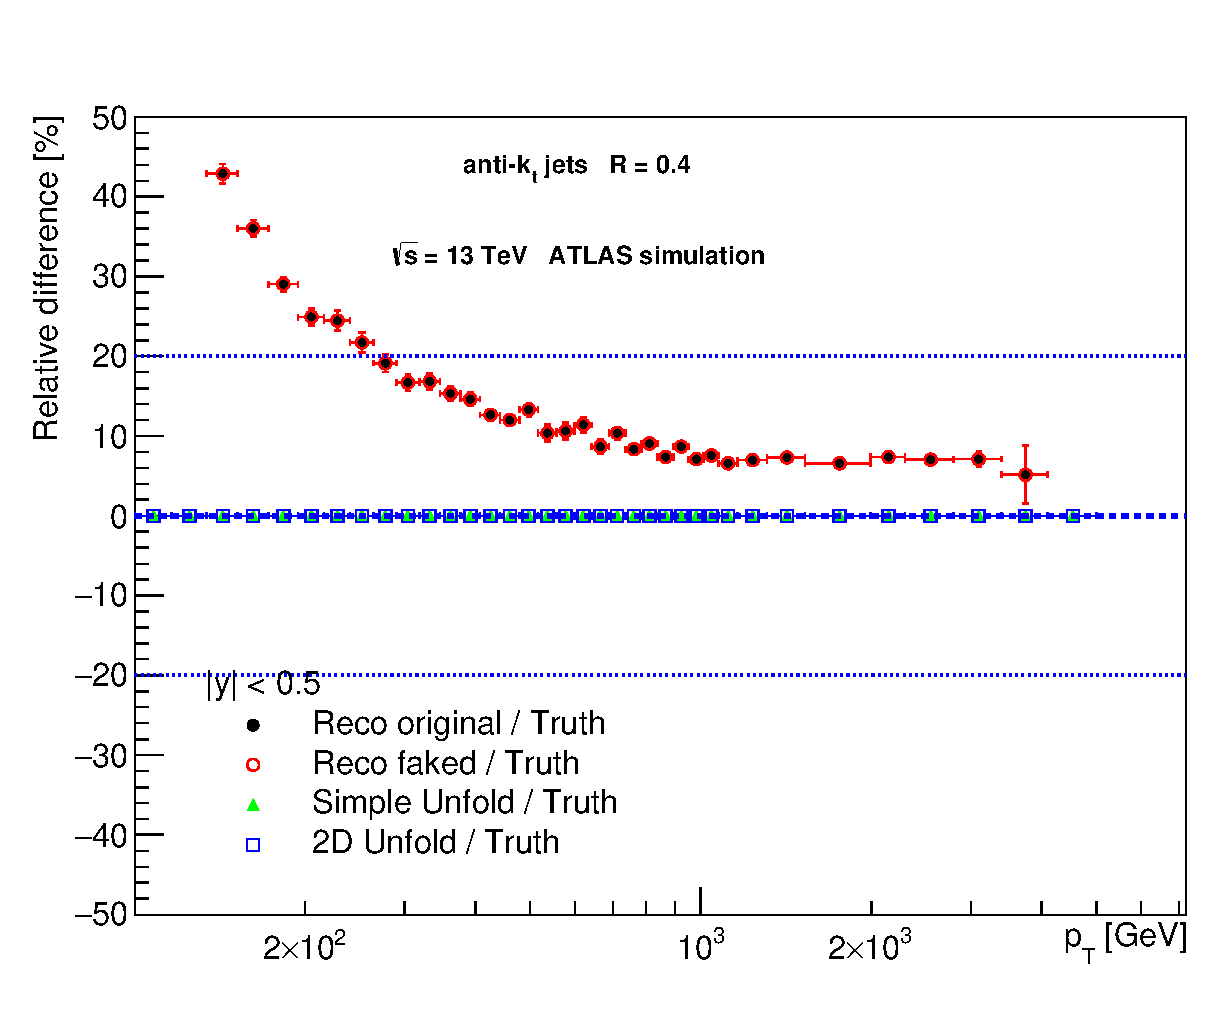
\includegraphics[width=0.33\textwidth]{FakedSignal0Compare.eps}
  \includegraphics[width=0.33\textwidth]{FakedSignal1Compare.eps}
  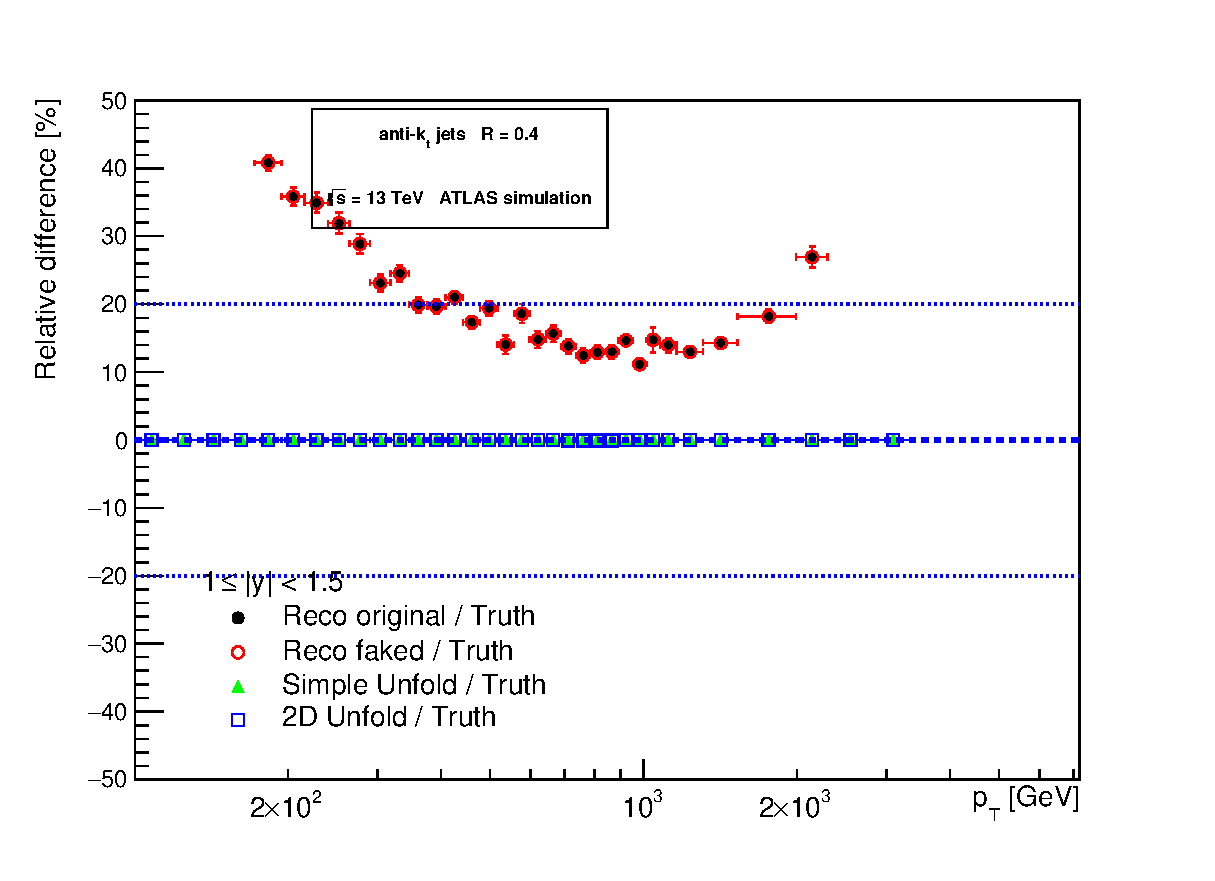
\includegraphics[width=0.33\textwidth]{FakedSignal2Compare.eps}

  \includegraphics[width=0.33\textwidth]{FakedSignalZoomed0Compare.eps}
  \includegraphics[width=0.33\textwidth]{FakedSignalZoomed1Compare.eps}
  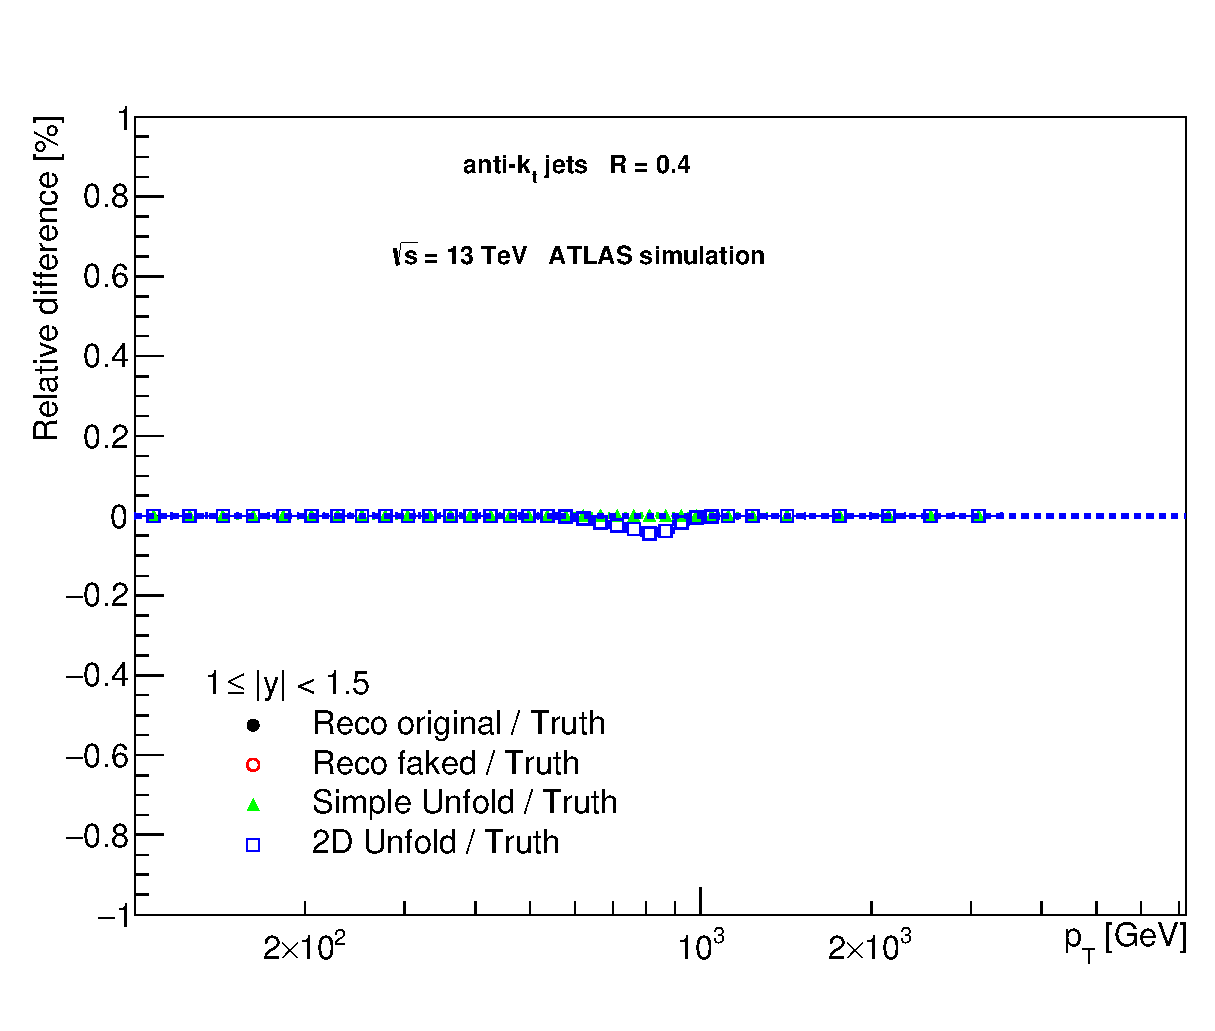
\includegraphics[width=0.33\textwidth]{FakedSignalZoomed2Compare.eps}
\end{figure}
\end{frame}

%------------------------------------------------

\begin{frame}
\frametitle{Conclusions}
\begin{block}{Matching Efficiencies}
  2D Unfolding: $> 99\,\%$ for almost every bin with $p_T>100\,\text{GeV}$.

  Simple Unfolding: $\sim 2-5\,\%$ worse.
\end{block}
\begin{block}{Unfolding Results}
  Small differences between both of these approaches.

  2D Unfolding: Small interconnection between neigboring rapidity bins

  Simple Unfolding: Interconnection is not possible
\end{block}
\end{frame}


%\begin{frame}
%\frametitle{Paragraphs of Text}
%Sed iaculis dapibus gravida. Morbi sed tortor erat, nec interdum arcu. Sed id lorem lectus. Quisque viverra augue id sem ornare non aliquam nibh tristique. Aenean in ligula nisl. Nulla sed tellus ipsum. Donec vestibulum ligula non lorem vulputate fermentum accumsan neque mollis.\\~\\
%
%Sed diam enim, sagittis nec condimentum sit amet, ullamcorper sit amet libero. Aliquam vel dui orci, a porta odio. Nullam id suscipit ipsum. Aenean lobortis commodo sem, ut commodo leo gravida vitae. Pellentesque vehicula ante iaculis arcu pretium rutrum eget sit amet purus. Integer ornare nulla quis neque ultrices lobortis. Vestibulum ultrices tincidunt libero, quis commodo erat ullamcorper id.
%\end{frame}
%
%%------------------------------------------------
%
%\begin{frame}
%\frametitle{Bullet Points}
%\begin{itemize}
%\item Lorem ipsum dolor sit amet, consectetur adipiscing elit
%\item Aliquam blandit faucibus nisi, sit amet dapibus enim tempus eu
%\item Nulla commodo, erat quis gravida posuere, elit lacus lobortis est, quis porttitor odio mauris at libero
%\item Nam cursus est eget velit posuere pellentesque
%\item Vestibulum faucibus velit a augue condimentum quis convallis nulla gravida
%\end{itemize}
%\end{frame}
%
%%------------------------------------------------
%
%\begin{frame}
%\frametitle{Blocks of Highlighted Text}
%\begin{block}{Block 1}
%Lorem ipsum dolor sit amet, consectetur adipiscing elit. Integer lectus nisl, ultricies in feugiat rutrum, porttitor sit amet augue. Aliquam ut tortor mauris. Sed volutpat ante purus, quis accumsan dolor.
%\end{block}
%
%\begin{block}{Block 2}
%Pellentesque sed tellus purus. Class aptent taciti sociosqu ad litora torquent per conubia nostra, per inceptos himenaeos. Vestibulum quis magna at risus dictum tempor eu vitae velit.
%\end{block}
%
%\begin{block}{Block 3}
%Suspendisse tincidunt sagittis gravida. Curabitur condimentum, enim sed venenatis rutrum, ipsum neque consectetur orci, sed blandit justo nisi ac lacus.
%\end{block}
%\end{frame}
%
%%------------------------------------------------
%
%\begin{frame}
%\frametitle{Multiple Columns}
%\begin{columns}[c] 
%
%\column{.45\textwidth} 
%\textbf{Heading}
%\begin{enumerate}
%\item Statement
%\item Explanation
%\item Example
%\end{enumerate}
%
%\column{.5\textwidth} % Right column and width
%Lorem ipsum dolor sit amet, consectetur adipiscing elit. Integer lectus nisl, ultricies in feugiat rutrum, porttitor sit amet augue. Aliquam ut tortor mauris. Sed volutpat ante purus, quis accumsan dolor.
%
%\end{columns}
%\end{frame}
%
%
%\begin{frame}
%\frametitle{Table}
%\begin{table}
%\begin{tabular}{l l l}
%\toprule
%\textbf{Treatments} & \textbf{Response 1} & \textbf{Response 2}\\
%\midrule
%Treatment 1 & 0.0003262 & 0.562 \\
%Treatment 2 & 0.0015681 & 0.910 \\
%Treatment 3 & 0.0009271 & 0.296 \\
%\bottomrule
%\end{tabular}
%\caption{Table caption}
%\end{table}
%\end{frame}
%
%%------------------------------------------------
%
%\begin{frame}
%\frametitle{Theorem}
%\begin{theorem}[Mass--energy equivalence]
%$E = mc^2$
%\end{theorem}
%\end{frame}
%
%%------------------------------------------------
%
%\begin{frame}[fragile] 
%\frametitle{Verbatim}
%\begin{example}[Theorem Slide Code]
%\begin{verbatim}
%\begin{frame}
%\frametitle{Theorem}
%\begin{theorem}[Mass--energy equivalence]
%$E = mc^2$
%\end{theorem}
%\end{frame}\end{verbatim}
%\end{example}
%\end{frame}
%
%%------------------------------------------------
%
%\begin{frame}
%\frametitle{Figure}
%Uncomment the code on this slide to include your own image from the same directory as the template .TeX file.
%%\begin{figure}
%%\includegraphics[width=0.8\linewidth]{test}
%%\end{figure}
%\end{frame}
%
%%------------------------------------------------
%
%\begin{frame}[fragile] % Need to use the fragile option when verbatim is used in the slide
%\frametitle{Citation}
%An example of the \verb|\cite| command to cite within the presentation:\\~
%
%This statement requires citation \cite{p1}.
%\end{frame}
%
%%------------------------------------------------
%
%\begin{frame}
%\frametitle{References}
%\footnotesize{
%\begin{thebibliography}{99} % Beamer does not support BibTeX so references must be inserted manually as below
%\bibitem[Smith, 2012]{p1} John Smith (2012)
%\newblock Title of the publication
%\newblock \emph{Journal Name} 12(3), 45 -- 678.
%\end{thebibliography}
%}
%\end{frame}
%
%%------------------------------------------------
%
%\begin{frame}
%\Huge{\centerline{The End}}
%\end{frame}

%----------------------------------------------------------------------------------------

\end{document} 
